\documentclass{article}

\usepackage[utf8]{inputenc}
\usepackage{graphicx}
\usepackage{amsmath}
\usepackage{amsfonts}
\usepackage{amssymb}
\usepackage{comment}
\usepackage{gensymb}
\usepackage{geometry}
\usepackage{float}
\usepackage{caption}
\usepackage{subcaption}
\usepackage{listings}
\usepackage{enumitem}

\geometry{a4paper, margin=1in}

\lstset{
    basicstyle=\ttfamily\small,
}

\title{CSCE 312 Lab 4}
\author{Oscar Leon, Kevin Lei, Rita Hernandez}

\date{March 10, 2024}


\begin{document}

\maketitle
\subsection*{\centering{Section 503}}

\section*{Problem 1}
\subsection*{Explanation of the System and its Connections}
To construct the enabling component of the IO, the control bus 8-bit input goes through two sets of AND gates (one for seeing if the read function must be enabled and the other for the write function). 
The address bus's 8-bit input (only the least significant four bits are considered as stated by the lab manual) goes through eight sets of AND gates to make sure only certain addresses are being accessed.
The result of the two AND gates (determining if the read or write operation should be enabled) and the eight AND gates (determining which address must be accessed) go through two sets of four AND gates.
The first set of AND gates represent whether an address will go through the read operation.
The second set of AND gates represent whether an address will go through the write operation.
Then, four D-Flip Flops are used (each corresponding to a certain output 00000101-00001000) with the enabling component being the output from the write AND gates.
A clock input was also included into the D-Flip Flops to ensure the memory aspect of the outputs are maintained.
The actual data going into the D-Flip Flops was from the data bus. In addition, four 8-bit inputs (00000001-00000100) go through a 4x2 mux which is used to select what the data bus should output.
The selector of the mux is the output of an encoder that has the four outputs from the four AND gates that makes sure that the read operation is enabled as well as that the certain address is chosen to be read. 

Based on the requirements illustrated in the Lab 4 manual, the memory was constructed by connecting a RAM and ROM with their corresponding inputs and outputs. 
The RAM has an 8-bit data input which is used as the data that can be written into the RAM for a corresponding memory address which is another input. 
The RAM also had a clock and a writing and output enable inputs. 
These enable inputs made sure that the writing and output operations only occurred when needed. 
In regards to the ROM, the only input was the memory address that needed to be read. 
The output was the data received from that address.

The CPU helped merge the system all together. 
A PC enabling input alongside a clock input was put into an AND gate. 
The output of the AND gate was used as the clock input for the IO system as well as the enabling signal for the RAM. 
The 8-bit control input was used as the control input for the IO unit. 
The control input is also put through a decoder with each output corresponding to a certain enabling control signal. 
These signals would go through the enable input for the tri-state data buffers in the data bus and address bus to ensure that the data would only be shared when needed. 
The address input was sent into the address input for the IO unit. It was also connected to the RAM and ROM through the data buffers mentioned earlier. 
The output of both of the memory components were sent through data buffers into a final output for the data that has been read. 
Likewise, the input of the data to be written goes into the RAM and the IO unit as inputs through data buffers. 

To expand more on how the connections were made in this system, multiple connections were established among all components, including the data bus. 
The system design was based on the Von Neumann architecture. 
Because of this, the connections between the CPU, memory, IO devices, and the databuses were established securely. 
A data bus serves as a vital connection for transmitting data between these system components. 
It is connected to the CPU, allowing data to be transferred to and from memory and IO devices. 
Additionally, the data buffers implemented were put to make sure that the signals in the bus were secure and accurate. 
The data buffer stores whatever data gets passed via the data bus. 
If no data gets passed, the buffer should store the previous value that was sent via this bus. 
The tri-state buffers will also help with not sending data when it is not needed (like when an enable signal is off).

\subsection*{Issues During the Lab}
In this lab, there were two main issues. 
The first issue in the lab was initially understanding the inputs required for the IO. 
However, by reviewing the requirements of the lab manual, the interpretation of the IO component was clarified. 
To fully verify that the system had the appropriate inputs and outputs, there were comprehensive checks to double check any inconsistencies in the output.

The second issue brought up was the absence of the PC enable input. 
Due to this restriction, the CPU did not correctly work. 
However, while debugging and reviewing the lab manual, the new insight of the PC input provided the solution of adding the PC enable input. 
By correcting this, the overall accuracy and functionality of the CPU within the system is ensured. 

\subsection*{Verification Methods}
To ensure that the five requirements were met, each component of the whole system was tested through different means.
To verify the accuracy of the data and address buses, we monitored their signals while performing various operations such as writing and reading data to and from the RAM, as well as transferring data between the microprocessor and the IO devices. 
By observing the buses, we made sure that the data was being properly transmitted correctly.
For the memory component, tests were conducted with different inputs to the memory unit. 
Then, the outputs were monitored to confirm that the data was accurately written to and retrieved from the RAM. 
Additionally, the ROM was confirmed to work as it received the designated data from the specified address inputs.
The IO system underwent thorough testing to ensure its functionality. 
The microprocessor was confirmed to work as it could address each input and output device individually, allowing for read and write operations to be performed accurately. 
By addressing each device, via the address and control buses, the accuracy of the IO system's communication with the microprocessor was confirmed.
Integration of the buses with the IO system was validated by testing the different control signals (numbered from 00000001 to 00000101). 
This ensured that data was transferred seamlessly between the microprocessor and IO devices, with each control signal performing its designated function effectively.
Overall, through systematic testing and observation of the system's behavior under various scenarios, the correctness and functionality of each requirement was verified, ensuring the precise operation of the system. 
Examples of the verification of the whole system are illustrated below with ten different configurations paired with their respective timing diagrams.

\begin{figure}[H]
    \centering
    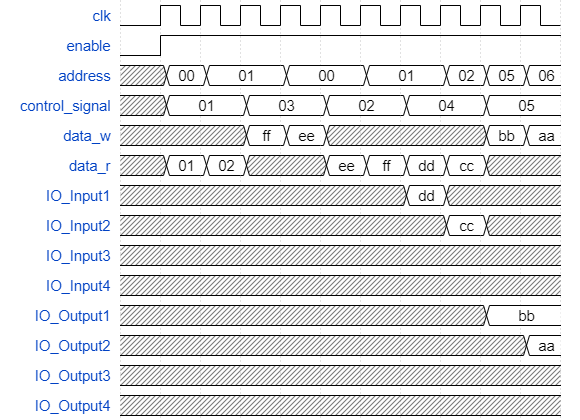
\includegraphics[width=0.8\textwidth]{./images/timing_diagram.png}
    \caption{Timing diagram for the system. Values are in hexadecimal.}
\end{figure}

\section*{Problem 2}
\subsection*{Adder}

\begin{figure}[H]
    \centering
    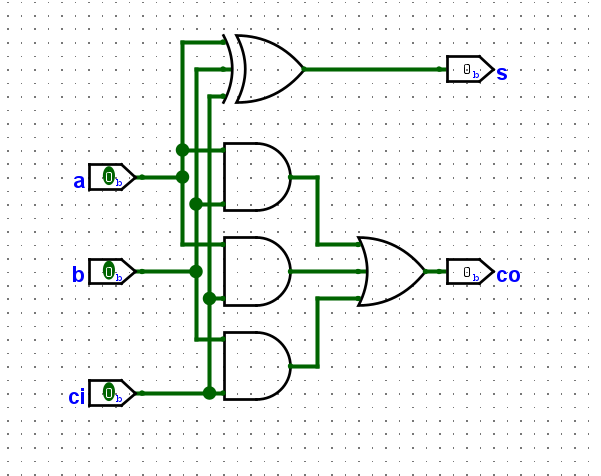
\includegraphics[width=0.5\textwidth]{./images/full_adder.png}
    \caption{Full adder.}
\end{figure}

\begin{figure}[H]
    \centering
    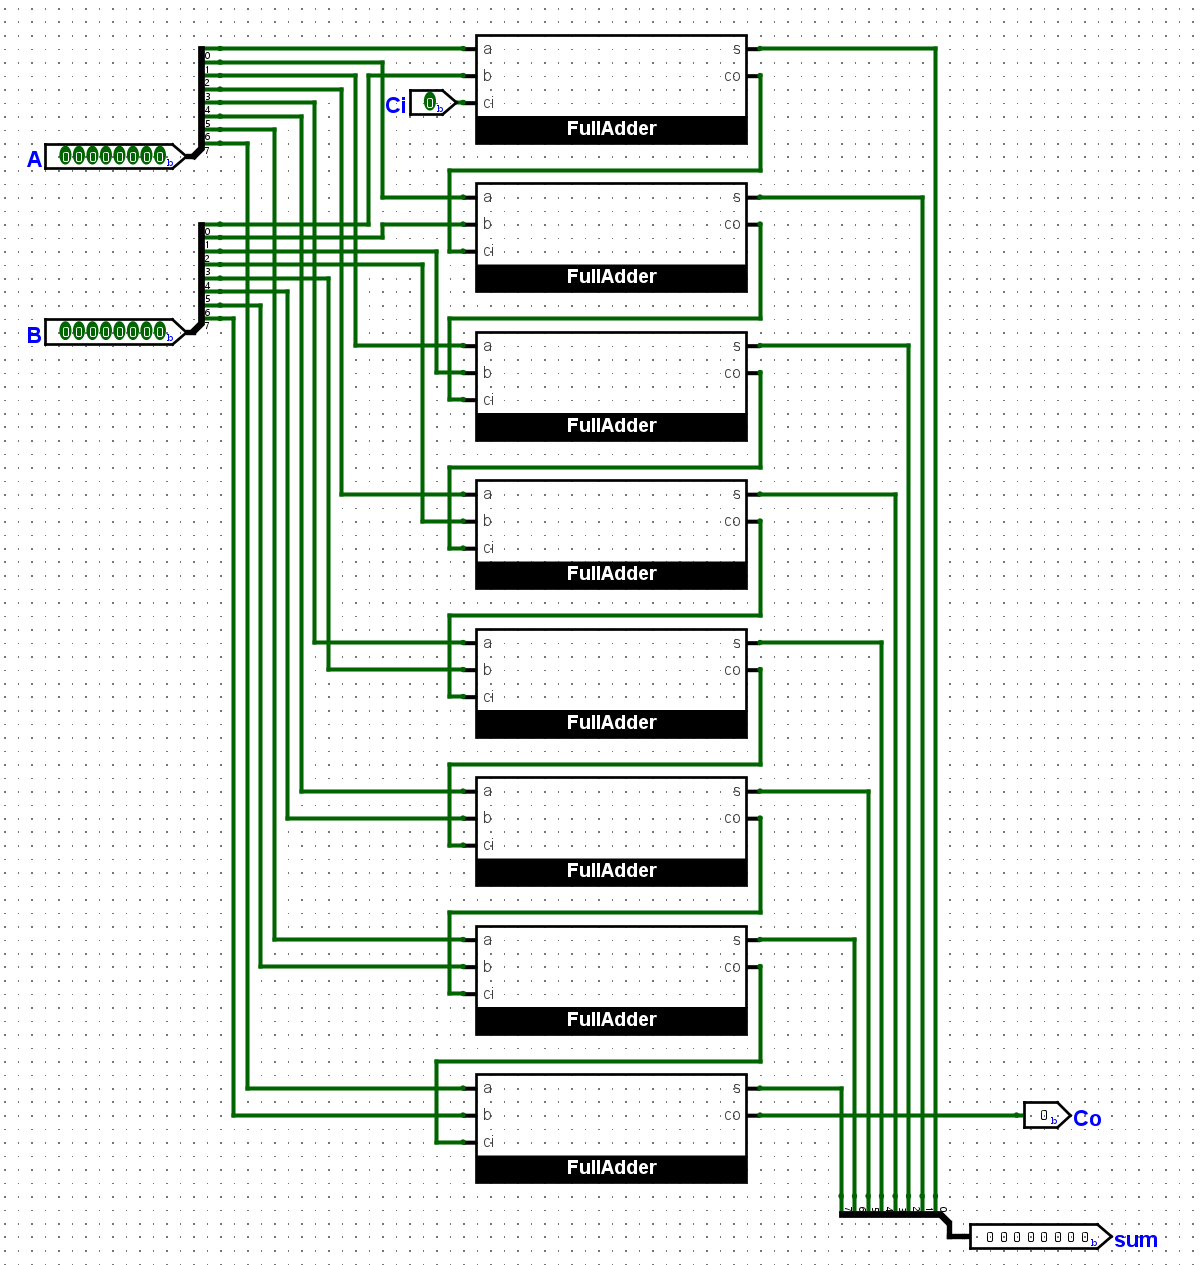
\includegraphics[width=0.75\textwidth]{./images/8-bit_full_adder.png}
    \caption{8-bit full adder.}
\end{figure}

\begin{figure}[H]
    \centering
    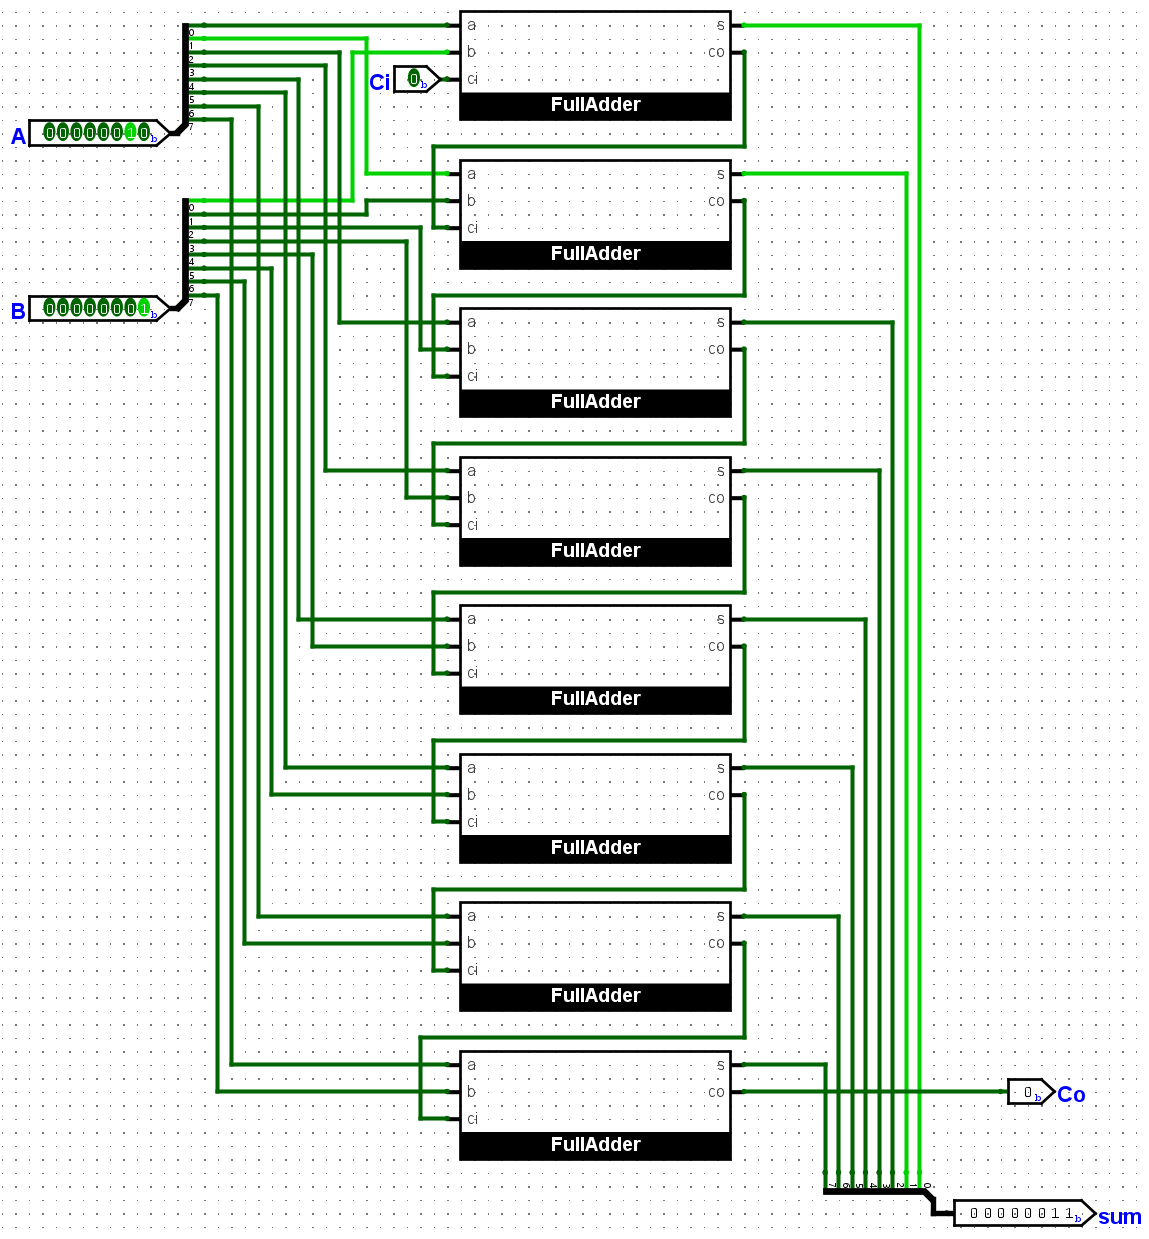
\includegraphics[width=0.8\textwidth]{./images/working_8-bit_full_adder.png}
    \caption{Working example of the 8-bit full adder shown in the previous figure.}
\end{figure}

\subsection*{Subtractor}

\begin{figure}[H]
    \centering
    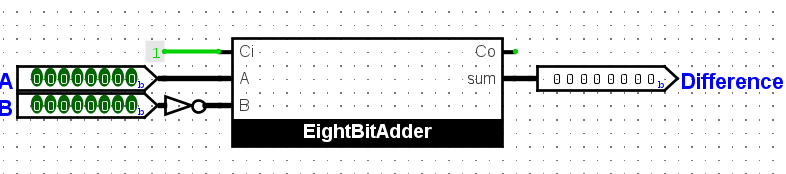
\includegraphics[width=0.8\textwidth]{./images/8-bit_subtractor.png}
    \caption{8-bit full subtractor using two's complement.}
\end{figure}

\begin{figure}[H]
    \centering
    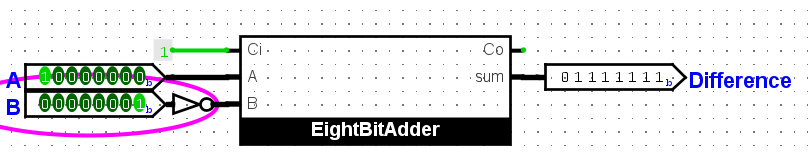
\includegraphics[width=0.8\textwidth]{./images/working_8-bit_subtractor.png}
    \caption{Working example of the 8-bit full subtractor shown in the previous figure.}
\end{figure}

\subsection*{Magnitude Comparator}

\begin{figure}[H]
    \centering
    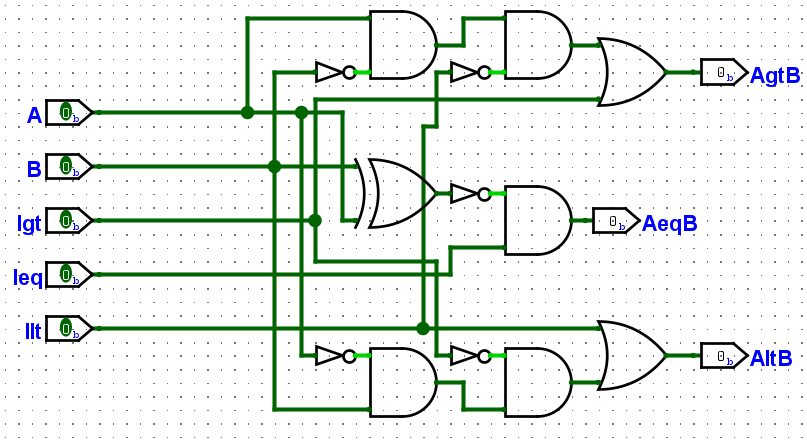
\includegraphics[width=0.5\textwidth]{./images/magnitude_comparator.png}
    \caption{Logic for the magnitude comparator.}
\end{figure}

\begin{figure}[H]
    \centering
    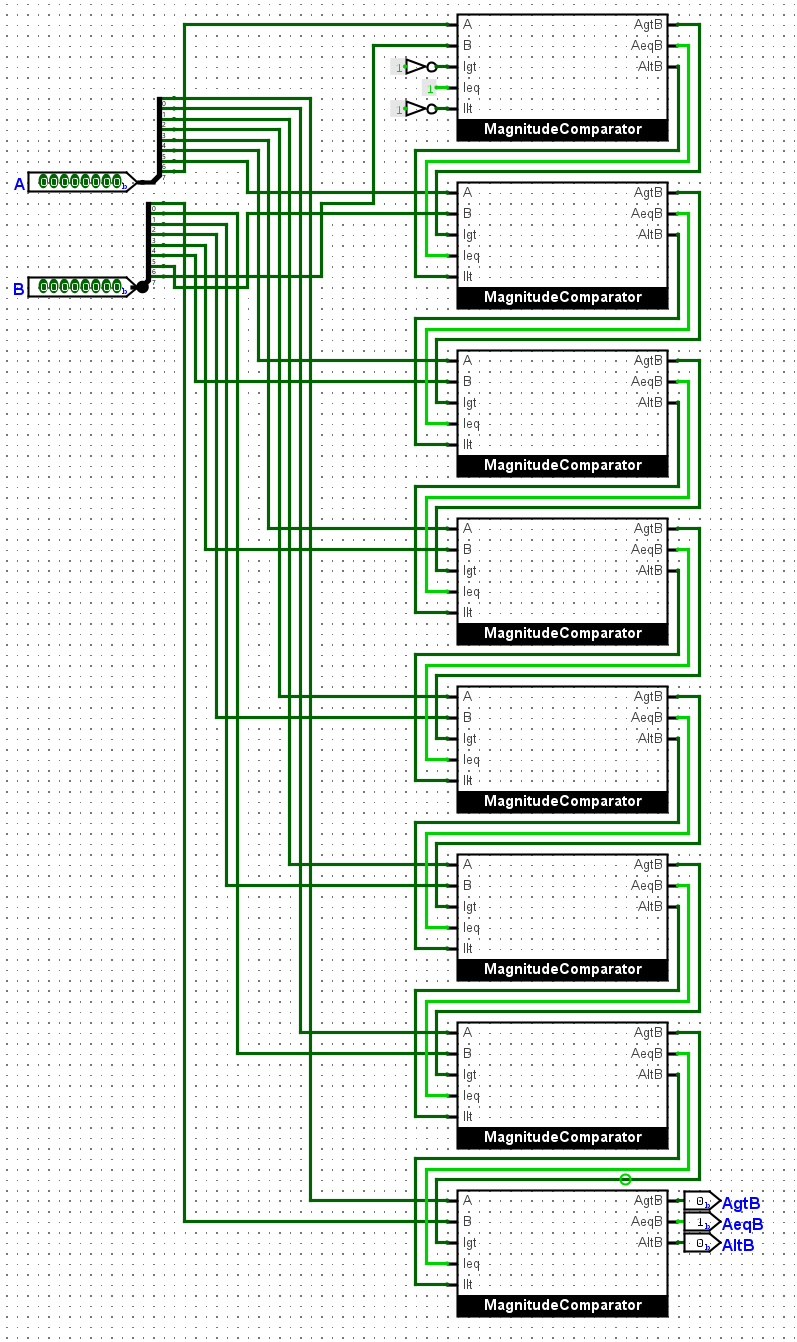
\includegraphics[width=0.6\textwidth]{./images/8-bit_comparator.png}
    \caption{8-bit magnitude comparator.}
\end{figure}

\begin{figure}[H]
    \centering
    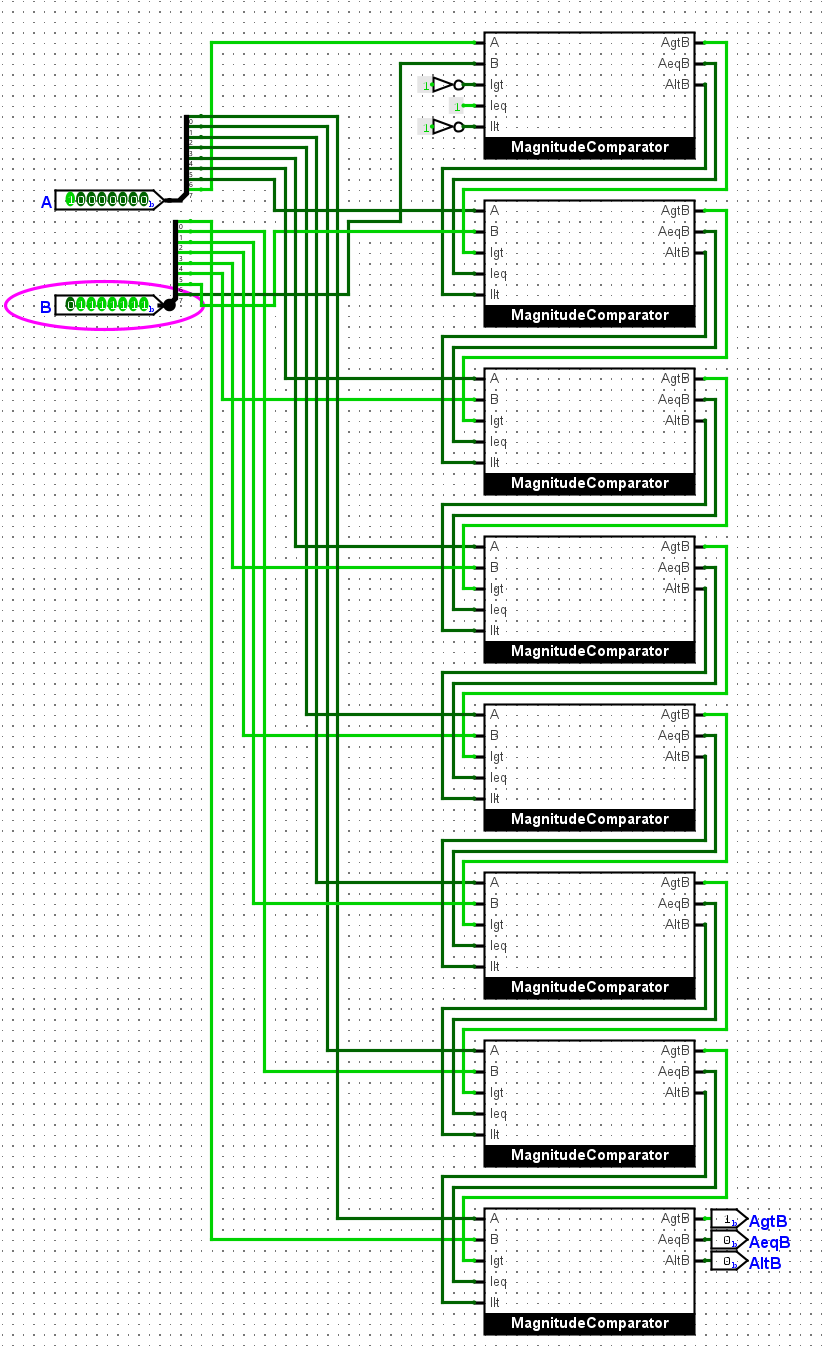
\includegraphics[width=0.8\textwidth]{./images/working_8-bit_comparator.png}
    \caption{Working example of the 8-bit magnitude comparator shown in the previous figure.}
\end{figure}

\subsection*{Left Barrel Shifter}

\begin{figure}[H]
    \centering
    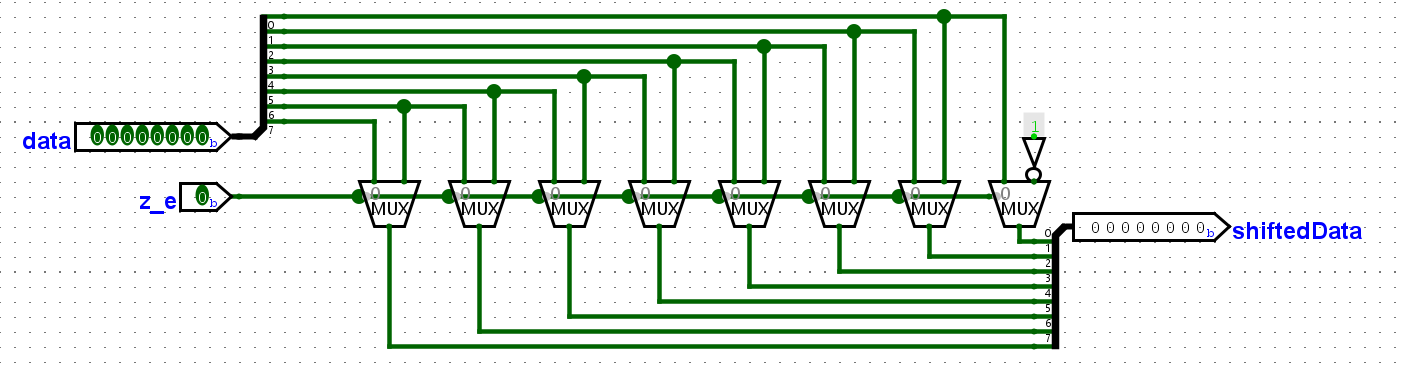
\includegraphics[width=0.6\textwidth]{./images/8-bit_single_left_sh.png}
    \caption{8-bit single left shifter.}
\end{figure}

\begin{figure}[H]
    \centering
    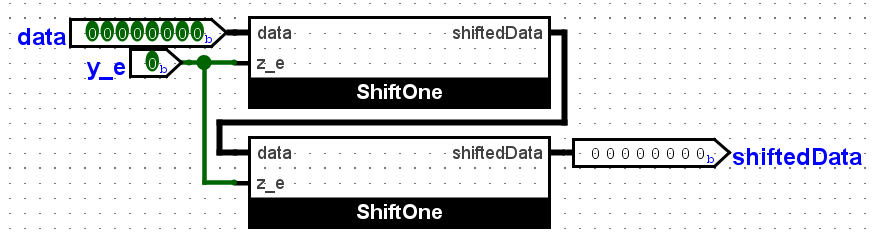
\includegraphics[width=0.6\textwidth]{./images/8-bit_double_left_sh.png}
    \caption{8-bit double left shifter.}
\end{figure}

\begin{figure}[H]
    \centering
    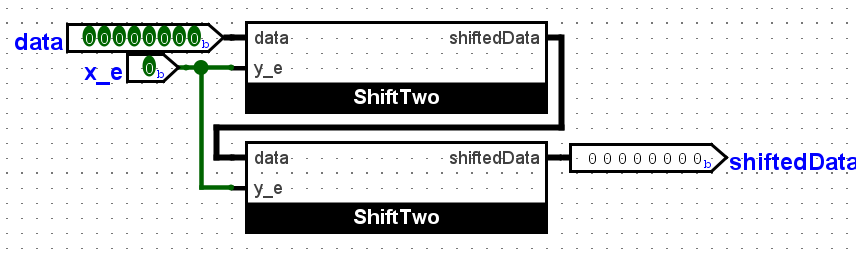
\includegraphics[width=0.6\textwidth]{./images/8-bit_quad_left_sh.png}
    \caption{8-bit quad left shifter.}
\end{figure}

\begin{figure}[H]
    \centering
    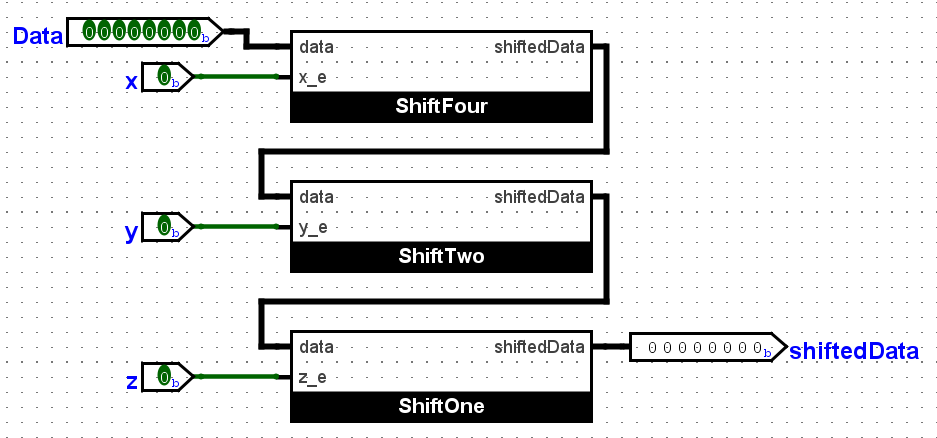
\includegraphics[width=0.6\textwidth]{./images/8-bit_full_left_sh.png}
    \caption{8-bit full left shifter.}
\end{figure}

\begin{figure}[H]
    \centering
    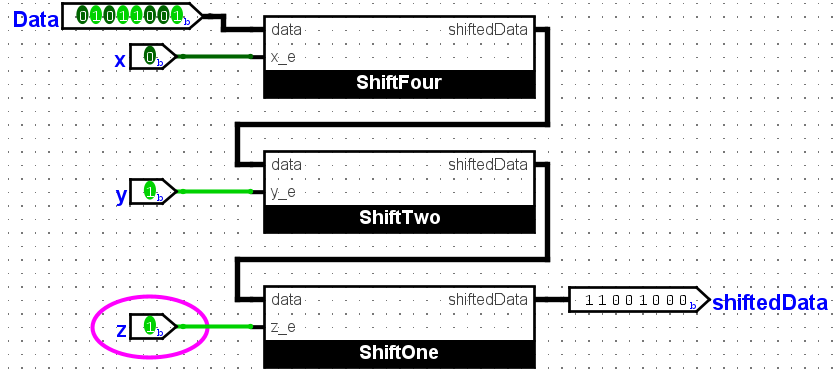
\includegraphics[width=0.6\textwidth]{./images/working_8-bit_full_left_sh.png}
    \caption{Working example of the 8-bit full left shifter shown in the previous figure.}
\end{figure}

\newpage
\section*{Problem 3}

\begin{figure}[H]
    \centering
    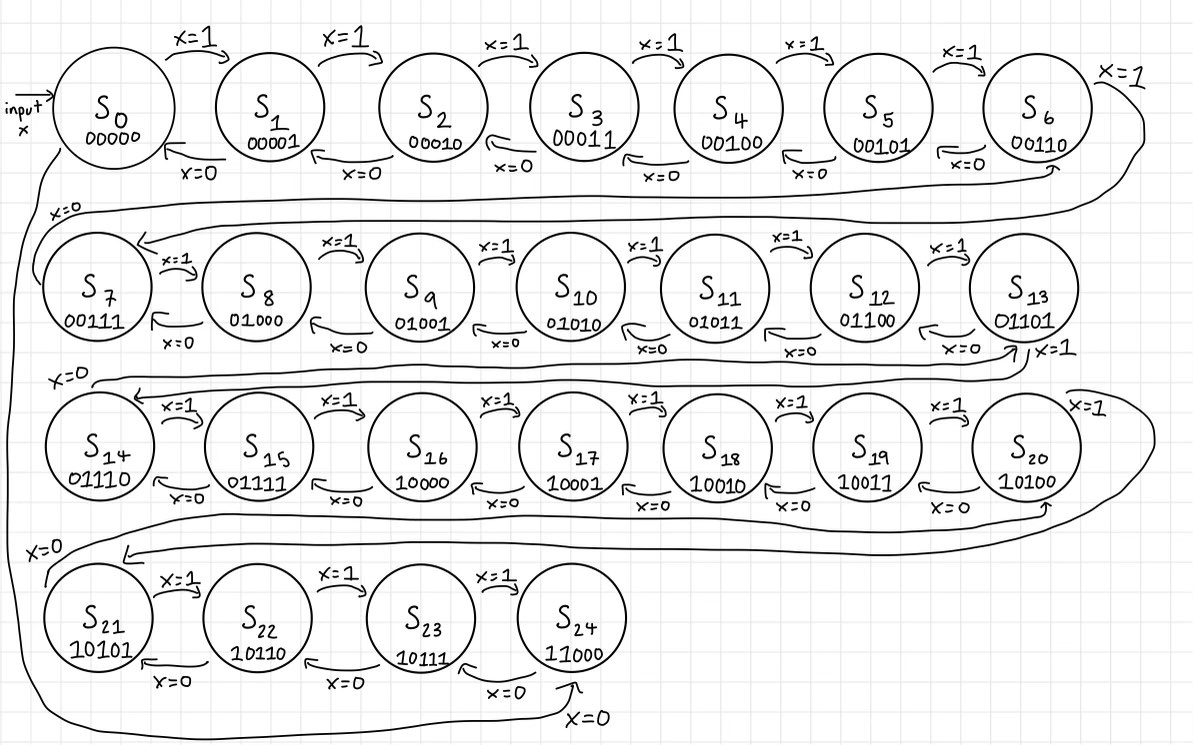
\includegraphics[width=0.8\textwidth]{./images/FSM.png}
    \caption{Finite State Machine for the LED display.}
\end{figure}

\begin{figure}[H]
    \centering
    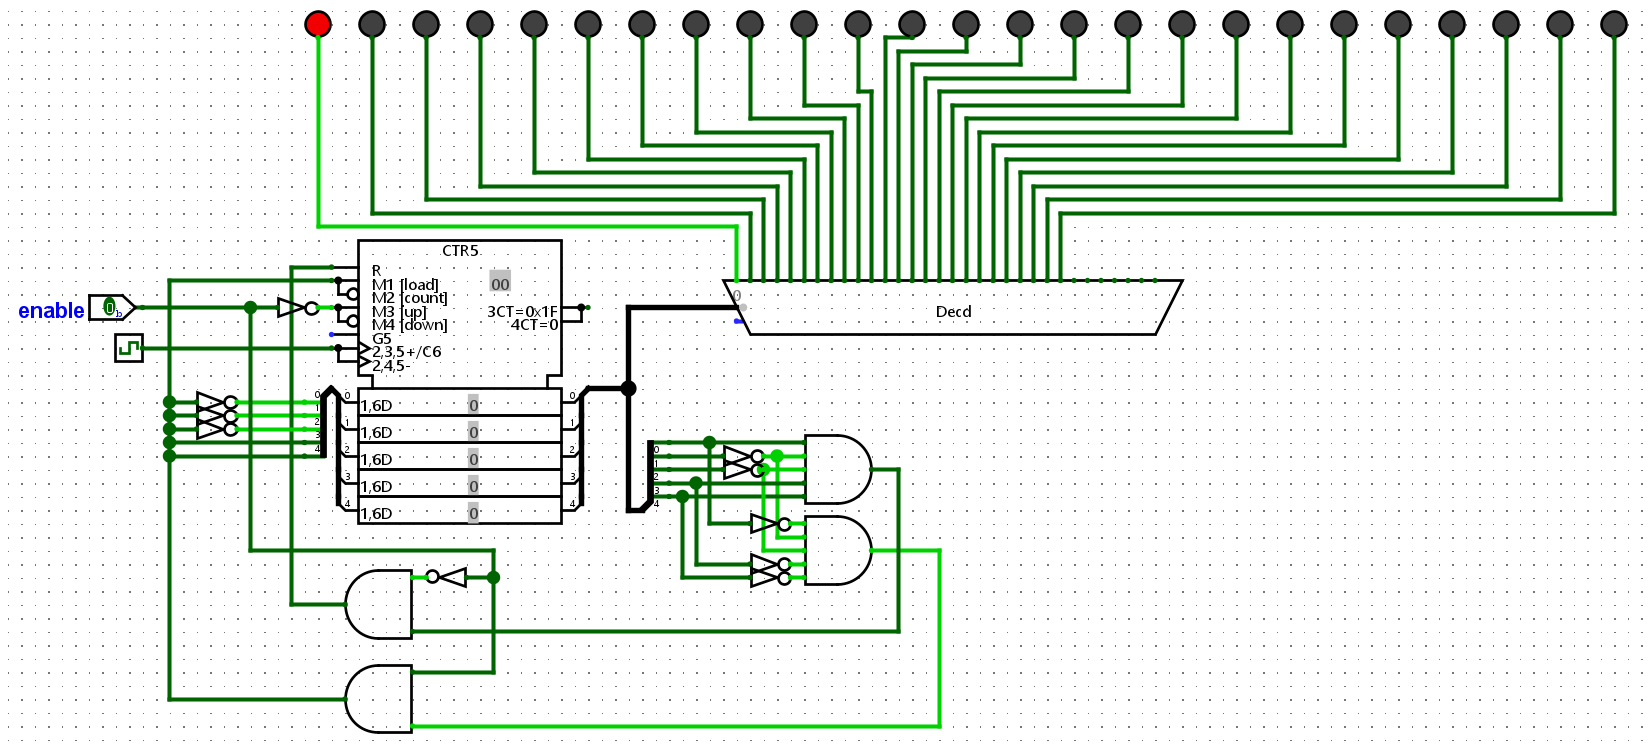
\includegraphics[width=0.8\textwidth]{./images/LED_decoder.png}
    \caption{LED display using a decoder.}
\end{figure}

\begin{figure}[H]
    \centering
    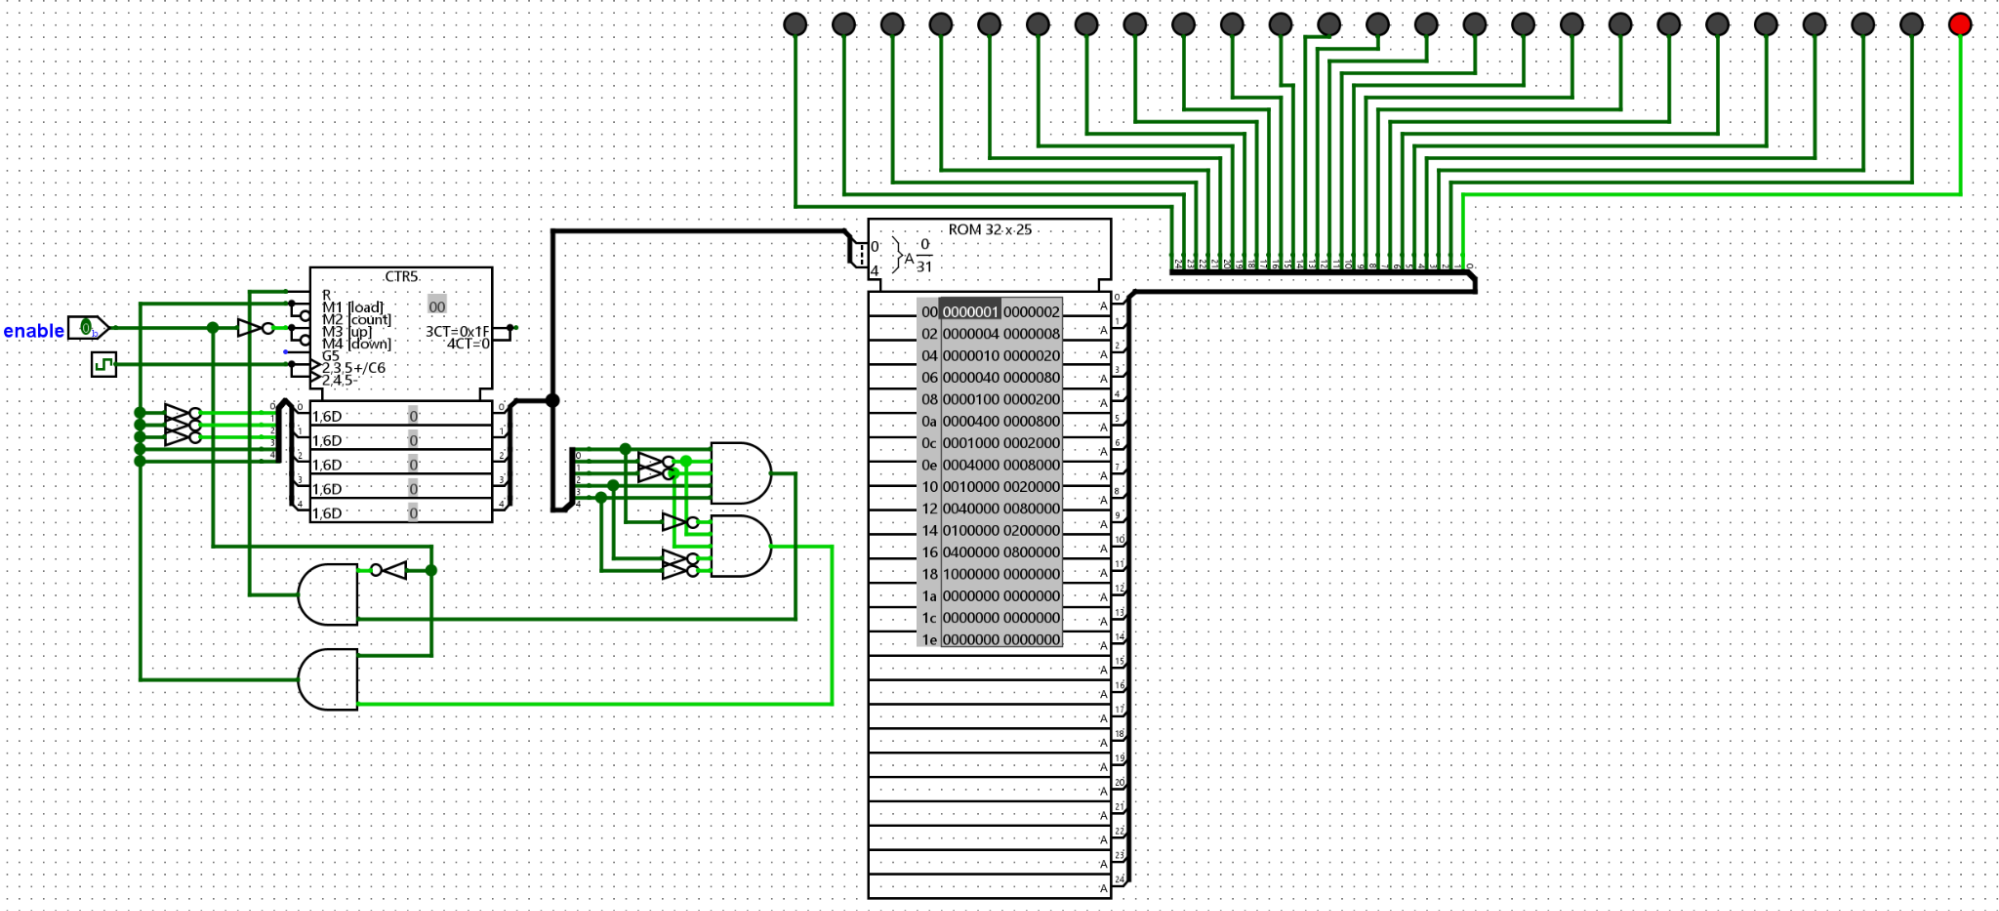
\includegraphics[width=0.8\textwidth]{./images/LED_ROM.png}
    \caption{LED display using a ROM.}
\end{figure}

\newpage
\section*{Appendix}
Oscar Leon was in charge of implementing the IO system in problem 1. He also designed the adder, subtractor, magnitude comparator, and the left-barrel shifter for problem 2. In addition, he developed the LED system using both a decoder and a ROM for problem 3.
Kevin Lei was in charge of creating the CPU and data/address bus component of problem 1. He also created the ten configurations of the system in problem 1, as well as their corresponding timing diagrams. 
Rita Hernandez Guerrero developed the memory component of problem 1. She also designed the Finite State Diagram for problem 3. 



\end{document}